\documentclass[a4paper,12pt]{article} 
\usepackage[utf8]{inputenc} % Acentos válidos sin problemas
\usepackage[spanish]{babel} % Idioma


\usepackage[backend=biber, style=alphabetic, sorting=ynt]{biblatex}
\bibliography{bibliografia.bib}
\nocite{*} % Añade todas las referencias de bib sin cita

%-----------------------------------INICIO DE PACKETES-------------------/
%-----------------------------------------------------------------------/
\usepackage{amsmath}   % Matemáticas: Comandos extras(cajas ecuaciones) |
\usepackage{amsthm}
\usepackage{amssymb}   % Matemáticas: Símbolos matemáticos              |
\usepackage{datetime}  % Agregar fechas                                 |
\usepackage{graphicx}  % Insertar Imágenes                              |
%\usepackage{biblatex} % Bibliografía                                   |
\usepackage{multicol}  % Creación de tablas                             |
\usepackage{longtable} % Tablas más largas                              |
\usepackage{xcolor}    % Permite cambiar colores del texto              |
\usepackage{tcolorbox} % Cajas de color                                 |
\usepackage{setspace}  % Usar espacios                                  |
\usepackage{fancyhdr}  % Para agregar encabezado y pie de página        |
\usepackage{lastpage}  %                                                 |
\usepackage{float}     % Flotantes                                      |
\usepackage{soul}      % "Efectos" en palabras                          |
\usepackage{hyperref}  % Para usar hipervínculos                        |
\usepackage{caption}   % Utilizar las referencias                       |
\usepackage{subcaption} % Poder usar subfiguras                         |
\usepackage{multirow}  % Nos permite modificar tablas                   |
\usepackage{array}     % Permite utilizar los valores para multicolumn  |
\usepackage{booktabs}  % Permite modificar tablas                       |
\usepackage{diagbox}   % Diagonales para las tablas                     |
\usepackage{colortbl}  % Color para tablas                              |
\usepackage{listings}  % Escribir código                               |
\usepackage{mathtools} % SIMBOLO :=                                     |
\usepackage{enumitem}  % Modificar items de Listas                      |
\usepackage{tikz}      %                                                |
\usepackage{lipsum}    % for auto generating text                       |
\usepackage{afterpage} % for "\afterpage"s                              |
\usepackage{pagecolor} % With option pagecolor={somecolor or none}|     |
\usepackage{xpatch}    % Color de lineas C & F
%\usepackage{glossaries} %                                              |
\usepackage{lastpage}    %                                              |   
\usepackage{csquotes}    %                                              |
%-----------------------------------------------------------------------\
%-----------------------------------FIN--- DE PACKETES-------------------\

\usepackage{pgfplots}     %                                             |
\pgfplotsset{compat=1.18} %           
\usepackage{etoolbox}
\usepackage{tikz,times}
\usepackage{verbatim}
\usetikzlibrary{mindmap,trees,backgrounds}
%--------------------------------/
%-------------------------------/
\usepackage[                 %   |
  headheight=15pt,  %            |
  letterpaper,  % Tipo de pag.   |
  left =1.5cm,  %  < 1 >         |
  right =1.5cm, %  < 1 >         | MARGENES DE LA PAGINA
  top =2cm,     %  < 1.5 >       |
  bottom =1.5cm %  < 1.5 >       |
]{geometry}     %                |
%-------------------------------\
%--------------------------------\

%----------------------------------------------------------------------/
%-------------------Encabezado y Pie de Pagina-----------------------/ |
%--------------------------------------------------------------------\ |
%\fancyhf{}
%\pagestyle{fancy}

\fancypagestyle{firstpage}{  
    \fancyhead[L]{}
    \fancyhead[R]{}     
    \fancyfoot[L]{}
    \fancyfoot[C]{}
    \fancyfoot[R]{\thepage\ de \pageref*{LastPage}}    
    \renewcommand{\headrulewidth}{0pt} 
    \xpretocmd\headrule{}{}{\PatchFailed}
}

\fancypagestyle{fancy}{  
    \fancyhead[L]{\textbf{Semestre: 2024-2}}
    \fancyhead[C]{}     
    \fancyhead[R]{}     

    \fancyfoot[L]{\texttt{Skynet Scribes}}
    \fancyfoot[C]{\texttt{IA}}
    \fancyfoot[R]{\thepage\ de \pageref*{LastPage}}

    \renewcommand{\headrulewidth}{1pt} 
    \xpretocmd\headrule{}{}{\PatchFailed}
    \renewcommand{\footrulewidth}{1.5pt} 
    \xpretocmd\footrule{}{}{\PatchFailed}
}

\fancypagestyle{fancyref}{  
    \fancyhead[L]{}
    \fancyhead[R]{}     
    \fancyfoot[L]{\texttt{Skynet Scribes}}
    \fancyfoot[C]{\texttt{IA}}
    \fancyfoot[R]{\thepage\ de \pageref*{LastPage}}    
    \renewcommand{\headrulewidth}{0pt} 
    \xpretocmd\headrule{}{}{\PatchFailed}
}
%--------------------------------------------------------------------\ |
%-------------------Encabezado y Pie de Pagina-----------------------/ |
%------------------------------------------------------------FIN----/


%--------------------------------------------------------------------/
%------------------- LISTA DE COLORES ------------------------------/ 
\definecolor{ProcessBlue}{RGB}{0,176,240}
\definecolor{NavyBlue}{RGB}{0,110,184}
\definecolor{Cyan}{RGB}{0,174,239}
\definecolor{MidnightBlue}{RGB}{0,103,49}
\definecolor{ForestGreen}{RGB}{0,155,85}
\definecolor{Goldenrod}{RGB}{255,223,66}
\definecolor{YellowGreen}{RGB}{152,204,112}
\definecolor{Sepia}{RGB}{103,24,0}
\definecolor{Peach}{RGB}{247,150,90}
\definecolor{CarnationPink}{RGB}{242,130,180}
\definecolor{Fuchsia}{RGB}{140,54,140}
\definecolor{WildStrawberry}{RGB}{238,41,103}
\definecolor{blueRY}{RGB}{13,164,245}

\definecolor{Grass}{RGB}{41,238,53}
\definecolor{Meadow}{RGB}{6,243,67}
\definecolor{jellyfish}{RGB}{109,14,130}
\definecolor{rubber}{RGB}{229,27,232}
\definecolor{bullet}{RGB}{225,31,90}
\definecolor{midnight}{RGB}{31,90,225}
\definecolor{sun}{RGB}{241,152,7}
\definecolor{water}{RGB}{16,229,183}

%------------------- COLORES CÓDIGO ---------------------- |
%------------------- COLORES JAVA ---------------------- |
\definecolor{backcolour}{RGB}{6,6,6} 
%\definecolor{backcolour}{RGB}{181,181,181} 
\definecolor{codeclassjava}{RGB}{246,113,59}
\definecolor{codegreen}{RGB}{17,225,48}
\definecolor{codenumizq}{RGB}{17,17,17}
\definecolor{codestringjava}{RGB}{51,240,234}
\definecolor{codesymboljava}{RGB}{255,5,0} 
\definecolor{yellowpoint}{RGB}{244,235,100} 
%------------------- COLORES JAVA ---------------------- |
%------------------- COLORES PYTHON -------------------- |
\definecolor{backcolourPY}{RGB}{6,6,6} 
%\definecolor{backcolour}{RGB}{181,181,181} 
\definecolor{codegreenPY}{RGB}{17,225,48}
\definecolor{codeclassPY}{RGB}{246,113,59}
\definecolor{codenumizq}{RGB}{17,17,17}
\definecolor{codestringPY}{RGB}{90,128,220}
\definecolor{codesymboljava}{RGB}{255,5,0} 
%------------------- COLORES PYTHON -------------------- |
%------------------- COLORES TERMINAL-------------------- |
\definecolor{backcolourTerminal}{rgb}{0.0, 0.0, 0.0} % Negro
\definecolor{codeclassTerminal}{rgb}{1.0, 1.0, 1.0} % Blanco
\definecolor{codestringTerminal}{rgb}{0.0, 0.6, 0.0} % Verde
\definecolor{codecommentTerminal}{rgb}{0.5, 0.5, 0.5} % Gris
\definecolor{codenumizqTerminal}{rgb}{0.0, 0.0, 1.0} % Azul
\definecolor{codeoptionTerminal}{rgb}{0.4, 0.4, 1.0} % Azul claro para opciones
\definecolor{yellowTerminal}{RGB}{238,200,62}
%------------------- COLORES TERMINAL-------------------- |
%------------------- COLORES CÓDIGO ---------------------- |



%------------------- LISTA DE COLORES -------------------------------\
%---------------------------------------------------------------------\

%-------------- ESTILO de Código PYTHON -----------------------------|
\lstdefinestyle{mystylepython}{
    backgroundcolor=\color{backcolourPY},
    commentstyle=\color{codecommentTerminal},
    keywordstyle=\color{blueRY},
    numberstyle=\tiny\color{codenumizq},
    stringstyle=\color{codestringPY},
    basicstyle=\footnotesize\ttfamily\color{white},
    breakatwhitespace=false,
    breaklines=true,
    captionpos=b,
    keepspaces=true,
    numbers=left,
    numbersep=5pt,
    showspaces=false,
    showstringspaces=false,
    showtabs=false,
    tabsize=2,
    escapechar=\&,
    literate=                
        {;}{{\textcolor{yellowpoint}{;}}}1
        {+}{{\textcolor{yellowpoint}{+}}}1
        {-}{{\textcolor{yellowpoint}{-}}}1
        {\{}{{\textcolor{yellowpoint}{\{}}}1
        {\}}{{\textcolor{yellowpoint}{\}}}}1
        {[}{{\textcolor{yellowpoint}{[}}}1
        {]}{{\textcolor{yellowpoint}{]}}}1
        {=}{{\textcolor{yellowpoint}{=}}}1
        {:}{{\textcolor{yellowpoint}{:}}}1
        {<}{{\textcolor{yellowpoint}{<}}}1
        {>}{{\textcolor{yellowpoint}{>}}}1
}
%-------------- ESTILO de Código PYTHON -----------------------------|
%-------------- ESTILO de Código TERMINAL ---------------------------|
\lstdefinestyle{mystyleTerminal}{
    backgroundcolor=\color{backcolourTerminal},
    commentstyle=\color{codecommentTerminal},
    keywordstyle=\color{codeclassTerminal},
    numberstyle=\tiny\color{backcolourTerminal},
    stringstyle=\color{codestringTerminal},
    basicstyle=\footnotesize\ttfamily\color{codeclassTerminal},
    breakatwhitespace=false,
    breaklines=true,
    captionpos=b,
    keepspaces=true,
    numbers=left,
    numbersep=5pt,
    showspaces=false,
    showstringspaces=false,
    showtabs=false,
    tabsize=4,    
    escapechar=\&,
    literate = 
            {--}{{\textcolor{codecommentTerminal}{--}}}2            
}
% Usar el estilo de código
\lstset{style=mystyleTerminal}
%-------------- ESTILO de Código TERMINAL ---------------------------|
\pagestyle{fancy}

\usepackage{algpseudocode}

\begin{document}%----------------------INICIO DOCUMENTO------------|
%------------------------------------------------------------------|
\begin{titlepage}
\center 
\newcommand{\HRule}{\rule{\linewidth}{0.5mm}} 

%---------------------
%	ESCUDO
%---------------------

\includegraphics[width=4.5cm]{IMA/cienciasWhite.png}

%----------------------------
%	TITULO
%----------------------------
\quad \\[0.2cm]
\textsc{\huge Facultad de Ciencias}\\[.6cm] 
\textsc{\huge Inteligencia Artificial}\\[0.5cm]

%-------------
%	TRABAJO
%-------------
\makeatletter
    \HRule \\ [0.4cm]
        { \huge \bfseries Exploradores de laberinto}\\
    \HRule \\ [0.4cm]
    
\vspace{2mm}

%----------------------------
%	Nombre del Equipo
%----------------------------
\begin{flushleft}
    \Large{Equipo:} \texttt{\Large Skynet Scribes}
\end{flushleft}
%----------------------------
%	Número de practica
%----------------------------
\begin{flushleft}
    \Large{Número de practica:} \texttt{\Large 02}\\[0.8cm]
\end{flushleft}


%-------------------
%	AUTORES
%-------------------
\begin{minipage}{0.8\textwidth}
    \begin{flushright}
        \textbf{\large{Carlos Daniel Cortés Jiménez}}\\    
        420004846        
    \end{flushright}
\end{minipage}

\vspace{5mm}

\begin{minipage}{0.4\textwidth}
        \textbf{\large{Sarah Sophía Olivares García}}\\
        318360638
\end{minipage}
\begin{minipage}{0.4\textwidth}
    \begin{flushright}
        \textbf{\large{Marco Silva Huerta}}\\
        316205326        
    \end{flushright}
\end{minipage}

\vspace{5mm}

\begin{minipage}{0.4\textwidth}
        \textbf{\large{Juan Daniel Barrera Holan}}\\    
        417079372
\end{minipage}
\begin{minipage}{0.4\textwidth}
    \begin{flushright}
        \textbf{\large{Laura Itzel Tinoco Miguel}}\\
        316020189
    \end{flushright}
\end{minipage}

\vspace{10mm}
%-------------------
%	PROFESORES
%-------------------

\begin{minipage}{0.8\textwidth}
    \begin{flushleft} \large
        Profesora: Cecilia Reyes Peña\\
        Ayudante teoría: Karem Ramos Calpulalpan \\
        Ayudante laboratorio: Tania Michelle Rubí Rojas\\                    
    \end{flushleft}
\end{minipage}

\vspace{20mm}

\begin{minipage}{0.4\textwidth}
    %---------------
    %	S E M E S T R E
    %---------------
    \textcolor{white}{Semestre}\\
    \large\textbf{Semestre 2024-2}      
\end{minipage}
\begin{minipage}{0.4\textwidth}
    %---------------
    %	F E C H A
    %---------------
    \begin{flushright}
        {\large Fecha de entrega:\\
         \textbf{28 de Febrero del 2024}}
    \end{flushright}
\end{minipage}

\makeatother

\vfill 
\end{titlepage}

\newpage
\tableofcontents

%% Investigación sobre el algoritmo
%\newpage
% ----------------------------------------------------------------------------------------\
% ---------------------------------------------------------------------------------------\
% --------------------------------------------------------------------------------------\
\section{Instrucciones}
% ----------------------------------------------------------------------------------------\
% ---------------------------------------------------------------------------------------\
% --------------------------------------------------------------------------------------\

\textbf{Problema a resolver:} Scheduling \\ 


\textbf{Objetivo:} Desarrollar e implementar un algoritmo genético para resolver 
el problema de asignación de horarios a profesores, asegurando que:

\begin{itemize}
    \item Los alumnos no tengan horas libres entre clases
    \item Los profesores no puedan tener dos clases al mismo tiempo
    \item Los salones no se asignen a dos grupos simultáneamente
    \item Los alumnos no tengan dos clases al mismo tiempo
\end{itemize}

% ----------------------------------------------------------------------------------------\
% ---------------------------------------------------------------------------------------\
% --------------------------------------------------------------------------------------\
\section{Investigación}
% ----------------------------------------------------------------------------------------\
% ---------------------------------------------------------------------------------------\
% --------------------------------------------------------------------------------------\

\subsubsection*{¿Qué es el algoritmo Genético?}

Un algoritmo genético \texttt{(AG)} entonces es: una técnica de resolución de problemas 
que utiliza principios inspirados en la selección natural para solucionar problemas de 
optimización. La selección natural (evolución) como estrategia implica la creación, 
reproducción y adaptación de una población de posibles soluciones en un rango de generaciones.\\ 

Este enfoque de población se basa en que cada individuo representa una posible solución 
al problema, y la evolución de estos comienza por, la \textbf{creación} de los individuos, 
la \textbf{reproducción} para después hacer la óptima \textbf{selección} de los padres en 
una nueva reproducción y \textbf{mutación}, finalmente comprobar o evaluar su \textbf{aptitud}\\ 


\subsubsection*{Pasos que sigue}

\begin{center}
    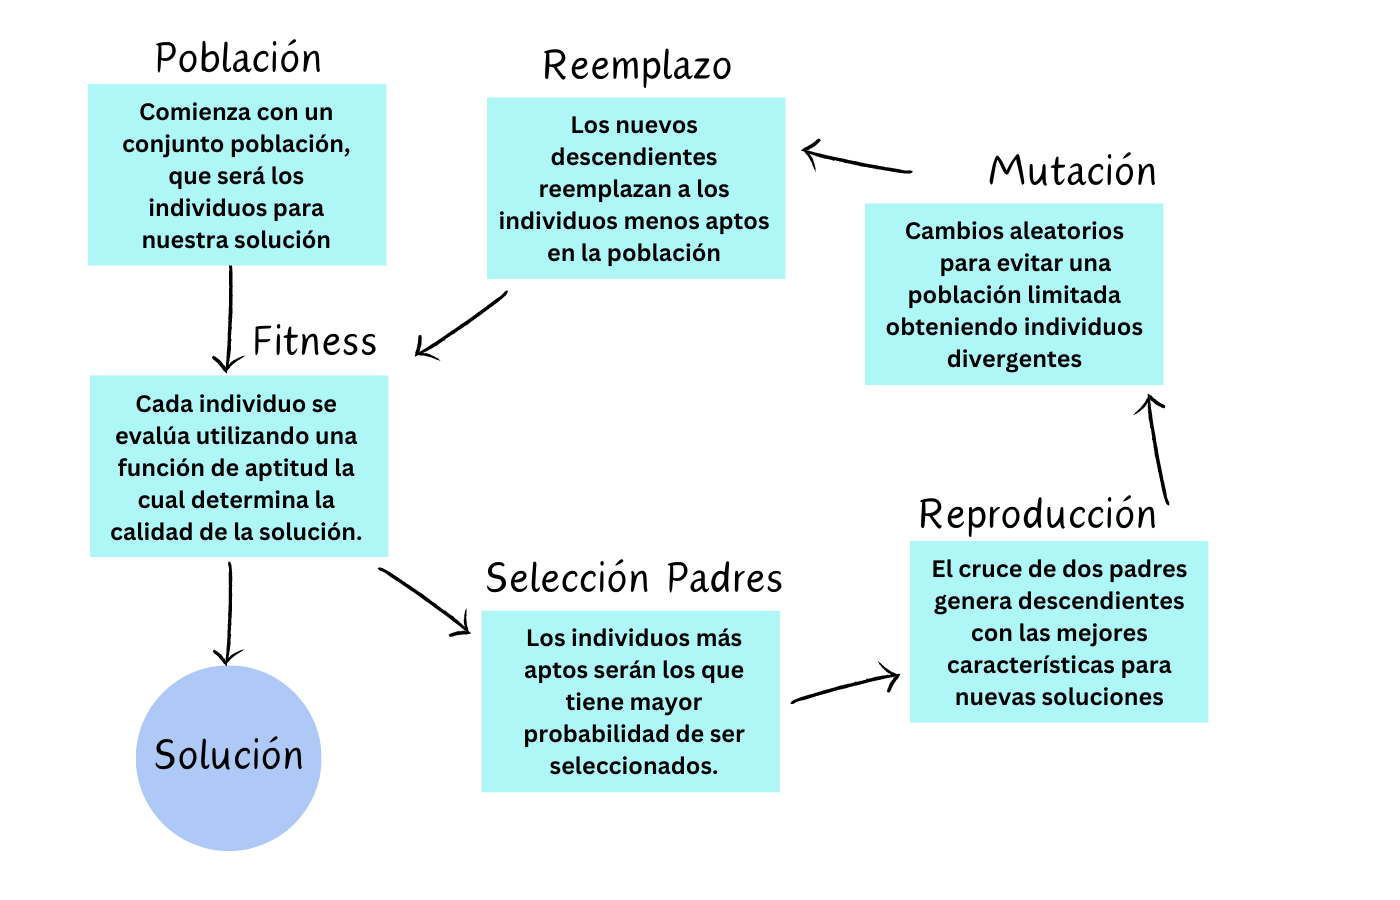
\includegraphics[scale = .4]{IMA/algo genetico.png}
\end{center}

\subsubsection*{Métodos de representación}

La definición de \texttt{(AG)} requiere de una función para codificar las soluciones 
potenciales del problema, de forma que el propio algoritmo pueda procesarlas aplicando las 
operaciones formales que le permiten evolucionar (\textbf{selección, reproducción y 
mutación}). Un enfoque común es codificar las soluciones como cadenas binarias: secuencias de 
$1's$ y $0's$, donde el dígito de cada posición representa la presencia/ausencia de algún 
aspecto de la solución.\cite{almosgenos} Algunas otras son:\\ 

\begin{itemize}
    \item \textbf{Representación Entera:} Los cromosomas son representados como secuencias 
    de enteros. Cada gen en el cromosoma representa un número entero que puede ser 
    interpretado como una característica, índice o valor en el espacio de búsqueda del problema

    \item \textbf{Representación Alfabética:} Los cromosomas son representados como secuencias 
    de elementos de un alfabeto prefijado. Aunque es equivalente a la representación entera, 
    es tan común que conviene identificarla como un método propio. Realmente, el resto de 
    representaciones se pueden interpretar como casos particulares de este, donde usaríamos 
    el alfabeto binario $(\{0,1\}), \text{entero} (\mathbb{Z}), \text{real} (\mathbb{R})$, etc.

    \item \textbf{Representación Permutacional:} Los cromosomas son representados como 
    permutaciones de un conjunto de elementos. Esta representación es útil para problemas en los 
    que la secuencia o el orden de los elementos son importantes, como en el problema del 
    agente viajero, donde el orden de las ciudades a visitar es crucial.

    \item \textbf{Representación Híbrida:} En algunos casos, se pueden utilizar múltiples tipos de 
    representaciones en un solo cromosoma. Por ejemplo, una parte del cromosoma puede ser binaria y 
    otra parte puede ser entera. Esto se hace para manejar diferentes tipos de variables en un problema 
    de optimización.
\end{itemize}

\subsubsection*{Métodos de selección}

\begin{itemize}
    \item \textbf{Selección elitista:} se garantiza la selección de los miembros más aptos de 
    cada generación.

    \item \textbf{Selección por rueda de ruleta:} una forma de selección proporcional a la aptitud 
    en la que la probabilidad de que un individuo sea seleccionado es proporcional a la diferencia 
    entre su aptitud y la de sus competidores.

    \item \textbf{Selección por torneo:} se eligen subgrupos de individuos de la población, y los 
    miembros de cada subgrupo compiten entre ellos. Sólo se elige a un individuo de cada subgrupo 
    para la reproducción.

    \item \textbf{Selección jerárquica:} los individuos atraviesan múltiples rondas de selección en 
    cada generación. Las evaluaciones de los primeros niveles son más rápidas y menos 
    discriminatorias, mientras que los que sobreviven hasta niveles más altos son evaluados 
    más rigurosamente. La ventaja de este método es que reduce el tiempo total de cálculo al 
    utilizar una evaluación más rápida y menos selectiva para eliminar a la mayoría de los 
    individuos que se muestran poco o nada prometedores, y sometiendo a una evaluación de aptitud 
    más rigurosa y computacionalmente más costosa solo a los que sobreviven a esta prueba inicial.
\end{itemize}

\subsubsection*{Métodos de reproducción}

Una vez que la selección ha elegido a los individuos aptos, estos deben mezclarse con el objetivo de 
conseguir nuevas soluciones, el método más habitual se basa en lo que se llama cruzamiento, y 
consiste en seleccionar a dos individuos para que intercambien segmentos de su código genético\\ 


Este proceso pretende simular el proceso análogo de la recombinación que se da en los cromosomas 
durante la reproducción sexual. Las formas comunes de cruzamiento incluyen:
\begin{itemize}
    \item Cruzamiento de un punto, en el que se establece un punto de intercambio en un lugar aleatorio 
    del genoma de los dos individuos, y uno de los individuos contribuye todo su código anterior a 
    ese punto y el otro individuo contribuye todo su código a partir de ese punto para producir 
    una descendencia.

    \item Cruzamiento en dos puntos, en el que se intercambian los genes que aparecen en el 
    intervalo de genes delimitados por dos puntos.

    \item Cruzamiento uniforme, en el que el valor de una posición dada en el genoma de la 
    descendencia corresponde al valor en esa posición del genoma de uno de los padres o al valor en 
    esa posición del genoma del otro padre, elegido con un $50\%$ de probabilidad.
\end{itemize}


\subsubsection*{Métodos de mutación}

Los métodos de mutación normalmente introducen cambios aleatorios en los individuos es un 
proceso que decide qué gen cambiará y qué valor tendrá tras la mutación esto con la 
esperanza de mejorar su aptitud para la siguiente generación. Al igual que las mutaciones 
en seres vivos causan cambios genéticos aleatorios, las mutaciones en algoritmos genéticos 
también provocan pequeñas alteraciones aleatorias en los cromosomas de los individuos.
%-------------------------------------------

%% Desarrollo sobre el trabajo realizado
%%  para las 3 partes del problema
%\newpage
% ----------------------------------------------------------------------------------------\
% ---------------------------------------------------------------------------------------\
% --------------------------------------------------------------------------------------\
\section{Desarrollo}
% ----------------------------------------------------------------------------------------\
% ---------------------------------------------------------------------------------------\
% --------------------------------------------------------------------------------------\
% Explicación de las implementaciones, diagrama de flujo, ideas, comentarios, investigación, etc
% ----------------------------------------------------------------------------------------\
% ---------------------------------------------------------------------------------------\
\subsection{Implementación básica del Juego de la Vida}
% ----------------------------------------------------------------------------------------\
% ---------------------------------------------------------------------------------------\



% ----------------------------------------------------------------------------------------\
% ---------------------------------------------------------------------------------------\
\subsection{Introducción a los Algoritmos Genéticos}
% ----------------------------------------------------------------------------------------\
% ---------------------------------------------------------------------------------------\



% ----------------------------------------------------------------------------------------\
% ---------------------------------------------------------------------------------------\
\subsection{Implementación de Algoritmos Genéticos en el Juego de la Vida}
% ----------------------------------------------------------------------------------------\
% ---------------------------------------------------------------------------------------\
%-------------------------------------------

%% Ilustración de las pruebas realizadas
%%  y punto extra final
% ----------------------------------------------------------------------------------------\
% ---------------------------------------------------------------------------------------\
% --------------------------------------------------------------------------------------\
\section{Resultados obtenidos}
% ----------------------------------------------------------------------------------------\
% ---------------------------------------------------------------------------------------\
% --------------------------------------------------------------------------------------\
% Mostrar ejecuciones del código con capturas 
% Mostrar una comparación del código

% ----------------------------------------------------------------------------------------\
% ---------------------------------------------------------------------------------------\
\subsection{Implementación básica del Juego de la Vida}
% ----------------------------------------------------------------------------------------\
% ---------------------------------------------------------------------------------------\




% ----------------------------------------------------------------------------------------\
% ---------------------------------------------------------------------------------------\
\subsection{Implementación de Algoritmos Genéticos en el Juego de la Vida}
% ----------------------------------------------------------------------------------------\
% ---------------------------------------------------------------------------------------\




% ----------------------------------------------------------------------------------------\
% ---------------------------------------------------------------------------------------\
% --------------------------------------------------------------------------------------\
\section{Reflexión final}
% ----------------------------------------------------------------------------------------\
% ---------------------------------------------------------------------------------------\
% --------------------------------------------------------------------------------------\

% Después de las simulaciones, analizar cómo la evolución de los cromosomas afectó el 
% desarrollo del Juego de la Vida, identificando patrones o estrategias exitosas.

% Redactar un breve informe que reflexione sobre el aprendizaje obtenido, las estrategias 
% que resultaron ser más efectivas y cómo los principios de los algoritmos genéticos 
% podrían aplicarse a otros problemas de optimización o simulación.
%-------------------------------------------


% ----------------------|
% Referencias           |
% Forma de Compilar     |
% pdflatex main.tex     |
% biber main            |
% pdflatex main.tex     |
\newpage %              |
\thispagestyle{fancyref}
\printbibliography %    |
% ----------------------|

\end{document}%----------------------F I N DOCUMENTO---------------|
%------------------------------------------------------------------|
